\chapter{Linked Lists}
\chaplabel{linkedlists}

In this chapter, we continue to study implementations of the #List#
interface, this time using pointer-based data structures rather than
arrays.  The structures in this chapter are made up of nodes that
contain the list items.  Using references (pointers) the nodes are
linked together into a sequence.  We first study singly-linked lists,
which can implement #Stack# and (FIFO) #Queue# operations in constant
time per operation and then move on to doubly-linked lists, which can
implement #Deque# operations in constant time.

Linked lists have advantages and disadvantages when compared to to array-based
implementations of the #List# interface.  The primary disadvantage is that
we lose the ability to access any element using #get(i)# or #set(i,x)#
in constant time.  Instead, we have to walk through the list, one element
at a time, until we reach the #i#th element.  The primary advantage is
that they are more dynamic:  Given a reference to any list node #u#, we
can delete #u# or insert a node adjacent to #u# in constant time. This
is true no matter where #u# is in the list.


\section{#SLList#: A Singly-Linked List}
\seclabel{sllist}

An #SLList# (singly-linked list) is a sequence of #Node#s.  Each node
#u# stores a data value #u.x# and a reference #u.next# to the next node in
the sequence.  For the last node #w# in the sequence, $#w.next# = #null#$

% TODO: Remove constructors from SLList.Node
\codeimport{ods/SLList.Node}

For efficiency, an #SLList# uses variables #head# and #tail# to keep
track of the first and last node in the sequence, as well as an integer
#n# to keep track of the length of the sequence:
\codeimport{ods/SLList.head.tail.n}
A sequence of #Stack# and #Queue# operations on an #SLList# is
illustrated in \figref{sllist}.

\begin{figure}
  \begin{center}
    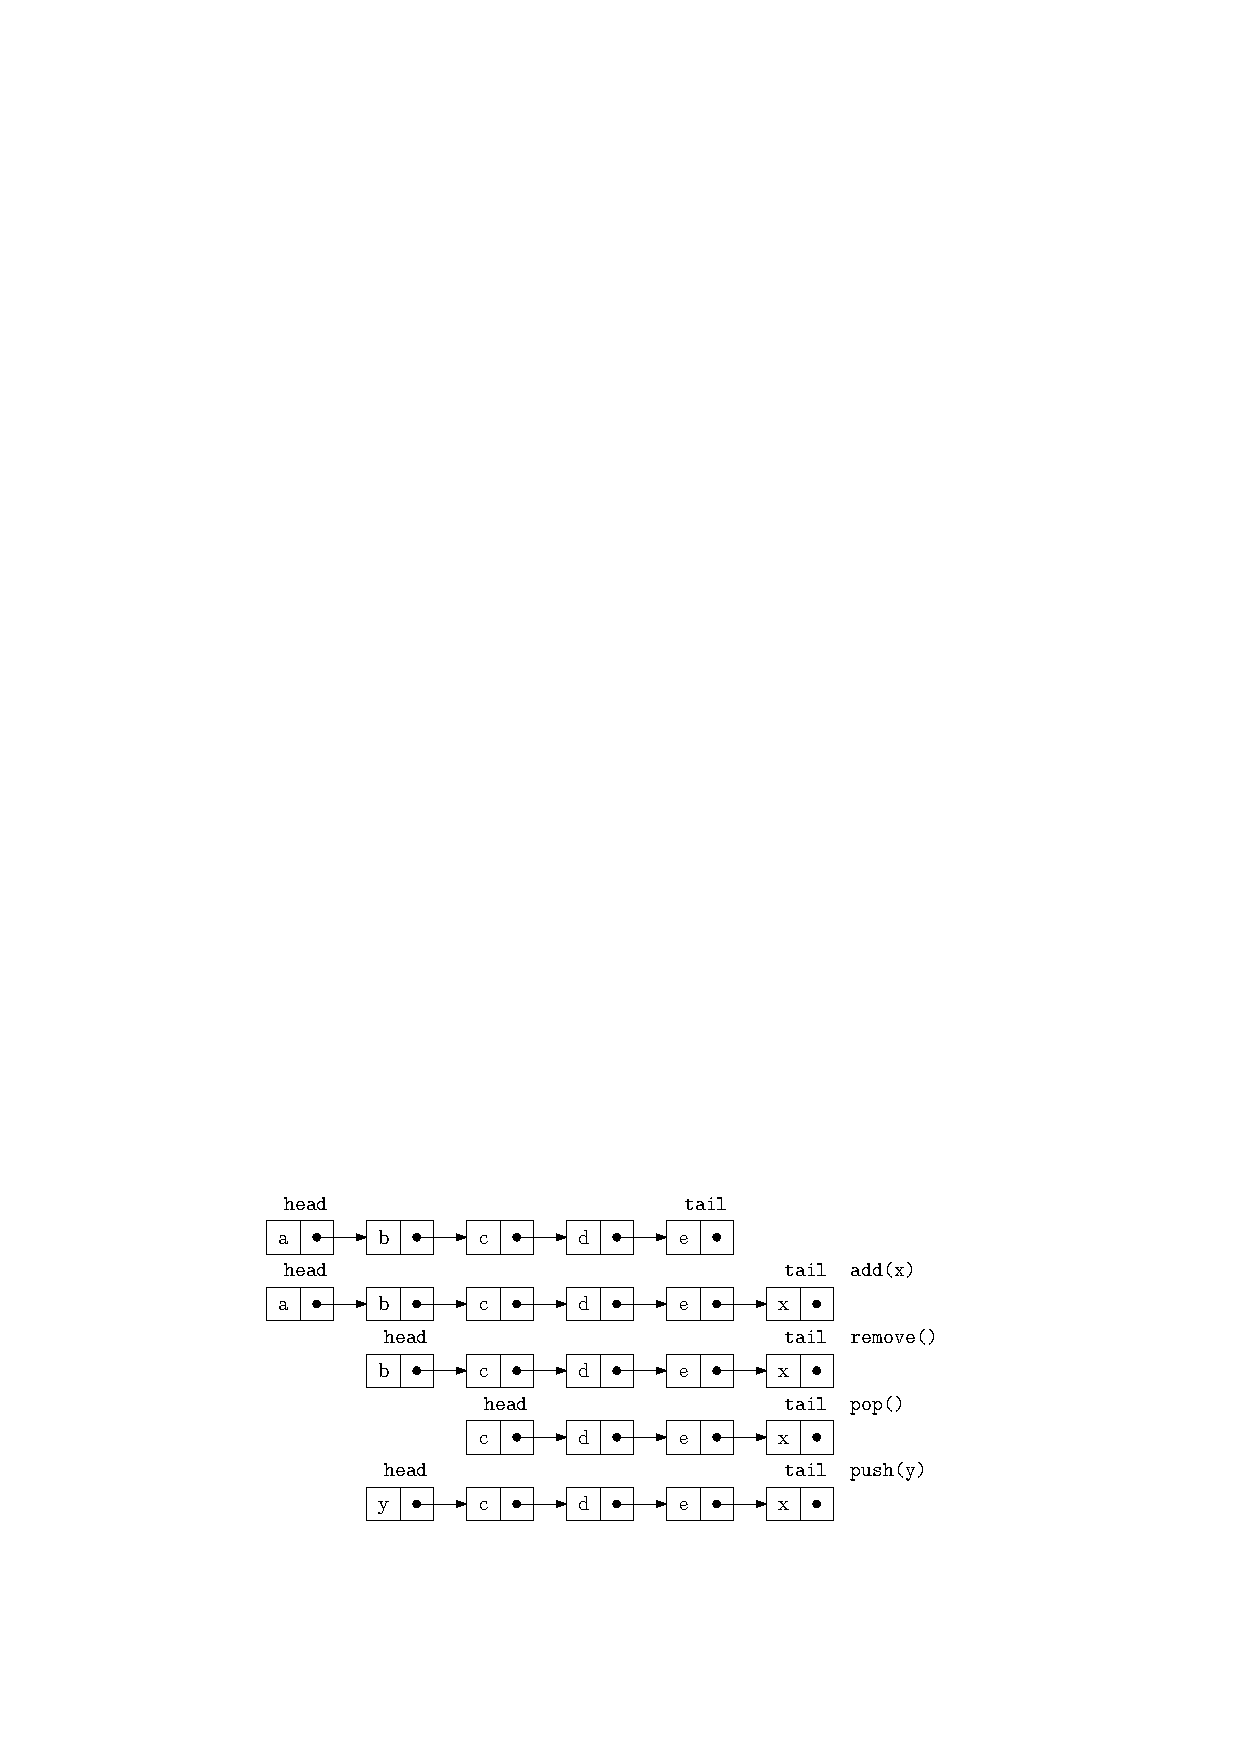
\includegraphics[width=\ScaleIfNeeded]{figs/sllist}
  \end{center}
  \caption[A sequence of Queue and Stack operations on an SLList]{A sequence of #Queue# (#add(x)# and #remove()#) and #Stack# (#push(x)# and #pop()#) operations on an #SLList#.}
  \figlabel{sllist}
\end{figure}


An #SLList# can efficiently implement the #Stack# operations #push()#
and #pop()# by adding and removing elements at the head of the sequence.
The #push()# operation simply creates a new node #u# with data value #x#,
sets #u.next# to the old head of the list and makes #u# the new head
of the list. Finally, it increments #n# since the size of the #SLList#
has increased by one:

\codeimport{ods/SLList.push(x)}

The #pop()# operation, after checking that the #SLList# is not empty,
removes the head by setting $#head#=#head.next#$ and decrementing #n#.
A special case occurs when the last element is being removed, in which case #tail# is set to #null#:

\codeimport{ods/SLList.pop()}

Clearly, both the #push(x)# and #pop()# operations run in $O(1)$ time.

\subsection{Queue Operations}

An #SLList# can also implement the FIFO queue operations #add(x)# and
#remove()# in constant time.  Removals are done from the head of the list,
and are identical to the #pop()# operation:

\codeimport{ods/SLList.remove()}

Additions, on the other hand, are done at the tail of the list.  In most
cases, this is done by setting $#tail.next#=#u#$, where #u# is the newly
created node that contains #x#.  However, a special case occurs when
$#n#=0$, in which case $#tail#=#head#=#null#$.  In this case, both #tail#
and #head# are set to #u#.

\codeimport{ods/SLList.add(x)}

Clearly, both #add(x)# and #remove()# take constant time.

\subsection{Summary}

The following theorem summarizes the performance of an #SLList#:

\begin{thm}\thmlabel{sllist}
  An #SLList# implements the #Stack# and (FIFO) #Queue# interfaces.  
  The #push(x)#, #pop()#, #add(x)# and #remove()# operations run
  in $O(1)$ time per operation.
\end{thm}

An #SLList# nearly implements the full set of #Deque# operations.
The only missing operation is removing from the tail of an #SLList#.
Removing from the tail of an #SLList# is difficult because it requires
updating the value of #tail# so that it points to the node #w#
that precedes #tail# in the #SLList#; this is the node #w# such that
$#w.next#=#tail#$.  Unfortunately, the only way to get to #w# is by
traversing the #SLList# starting at #head# and taking $#n#-2$ steps.

\section{#DLList#: A Doubly-Linked List}
\seclabel{dllist}

A #DLList# (doubly-linked list) is very similar to an #SLList# except
that each node #u# in a #DLList# has references to both the node #u.next#
that follows it and the node #u.prev# that precedes it.

\codeimport{ods/DLList.Node}

When implementing an #SLList#, we saw that there were always several
special cases to worry about. For example, removing the last element
from an #SLList# or adding an element to an empty #SLList# requires care
to ensure that #head# and #tail# are correctly updated.  In a #DLList#,
the number of these special cases increases considerably.  Perhaps the
cleanest way to take care of all these special cases in a #DLList# is to
introduce a #dummy# node. This is a node that does not contain any data,
but acts as a placeholder so that there are no special nodes; every node
has both a #next# and a #prev#, with #dummy# acting as the node that
follows the last node in the list and that precedes the first node in
the list.  In this way, the nodes of the list are (doubly-)linked into
a cycle, as illustrated in \figref{dllist}.

\begin{figure}
  \begin{center}
    \includegraphics[width=\ScaleIfNeeded]{figs/dllist2}
  \end{center}
  \caption[A DLList]{A #DLList# containing a,b,c,d,e.}
  \figlabel{dllist}
\end{figure}


%TODO: Remove constructors from class Node

\codeimport{ods/DLList.n.dummy.DLList()}

Finding the node with a particular index in a #DLList# is easy;  we can
either start at the head of the list (#dummy.next#) and work forward,
or start at the tail of the list (#dummy.prev#) and work backward.
This allows us to reach the #i#th node in $O(1+\min\{#i#,#n#-#i#\})$ time:

\codeimport{ods/DLList.getNode(i)}

The #get(i)# and #set(i,x)# operations are now also easy.  We first find the #i#th node and then get or set its #x# value:

\codeimport{ods/DLList.get(i).set(i,x)}

The running time of these operations is dominated by the time it takes
to find the #i#th node, and is therefore $O(1+\min\{#i#,#n#-#i#\})$.

\subsection{Adding and Removing}

If we have a reference to a node #w# in a #DLList# and we want to insert a
node #u# before #w#, then this is just a matter of setting $#u.next#=#w#$,
$#u.prev#=#w.prev#$, and then adjusting #u.prev.next# and #u.next.prev#.  (See \figref{dllist-addbefore}.)
Thanks to the dummy node, there is no need to worry about #w.prev#
or #w.next# not existing.

\codeimport{ods/DLList.addBefore(w,x)}

\begin{figure}
   \begin{center}
      \includegraphics[scale=0.90909]{figs/dllist-addbefore}
   \end{center}
   \caption[Adding to a DLList]{Adding the node #u# before the node #w#
      in a #DLList#.}
   \figlabel{dllist-addbefore}
\end{figure}

Now, the list operation #add(i,x)# is trivial to implement.  We find the
#i#th node in the #DLList# and insert a new node #u# that contains #x#
just before it.

\codeimport{ods/DLList.add(i,x)}

The only non-constant part of the running time of #add(i,x)# is the time
it takes to find the #i#th node (using #getNode(i)#).  Thus, #add(i,x)#
runs in $O(1+\min\{#i#, #n#-#i#\})$ time.

Removing a node #w# from a #DLList# is easy.  We need only adjust pointers
at #w.next# and #w.prev# so that they skip over #w#.  Again, the use of the dummy node eliminates the need to consider any special cases:

\codeimport{ods/DLList.remove(w)}

Now the #remove(i)# operation is trivial. We find the node with index #i# and remove it:

\codeimport{ods/DLList.remove(i)}

Again, the only expensive part of this operation is finding the #i#th node
using #getNode(i)#, so #remove(i)# runs in $O(1+\min\{#i#, #n#-#i#\})$
time.

\subsection{Summary}

The following theorem summarizes the performance of a #DLList#:

\begin{thm}\thmlabel{dllist}
  A #DLList# implements the #List# interface.  In this implementation,
  the #get(i)#, #set(i,x)#, #add(i,x)# and #remove(i)# operations run
  in $O(1+\min\{#i#,#n#-#i#\})$ time per operation.
\end{thm}

It is worth noting that, if we ignore the cost of the #getNode(i)#
operation, then all operations on a #DLList# take constant time.
Thus, the only expensive part of operations on a #DLList# is finding
the relevant node.  Once we have the relevant node, adding, removing,
or accessing the data at that node takes only constant time.

This is in sharp contrast to the array-based #List# implementations of
\chapref{arrays}; in those implementations, the relevant array
item can be found in constant time. However, addition or removal requires
shifting elements in the array and, in general, takes non-constant time.

For this reason, linked list structures are well-suited to applications
where references to list nodes can be obtained through external means.
\javaonly{An example of this is the #LinkedHashSet# data structure found in the
Java Collections Framework, in which a set of items is stored in a
doubly-linked list and the nodes of the doubly-linked list are stored
in a hash table (discussed in \chapref{hashing}).  When elements
are removed from a #LinkedHashSet#, the hash table is used to find the
relevant list node in constant time and then the list node is deleted
(also in constant time).}
\cpponly{For example, pointers to the nodes of a linked list could be
stored in a #USet#.  Then, to remove an item #x# from the linked list,
the node that contains #x# can be found quickly using the #Uset# and
the node can be removed from the list in constant time.}

\section{#SEList#: A Space-Efficient Linked List}
\seclabel{selist}

One of the drawbacks of linked lists (besides the time it takes to access
elements that are deep within the list) is their space usage.  Each node
in a #DLList# requires an additional two references to the next and
previous nodes in the list.  Two of the fields in a #Node# are dedicated
to maintaining the list, and only one of the fields is for storing data!

An #SEList# (space-efficient list) reduces this wasted space using
a simple idea: Rather than store individual elements in a #DLList#,
we store a block (array) containing several items. More precisely, an
#SEList# is parameterized by a \emph{block size} #b#. Each individual
node in an #SEList# stores a block that can hold up to #b+1# elements.

For reasons that will become clear later, it will be helpful if we
can do #Deque# operations on each block.  The data structure we choose
for this is a #BDeque# (bounded deque), derived from the #ArrayDeque#
structure described in \secref{arraydeque}.  The #BDeque# differs from the
#ArrayDeque# in one small way: When a new #BDeque# is created, the size
of the backing array #a# is fixed at #b+1# and never grows or shrinks.
The important property of a #BDeque# is that it allows for the addition
or removal of elements at either the front or back in constant time. This
will be useful as elements are shifted from one block to another.


\codeimport{ods/SEList.BDeque}

An #SEList# is then a doubly-linked list of blocks:

\codeimport{ods/SEList.Node}
\codeimport{ods/SEList.n.dummy}

\subsection{Space Requirements}

An #SEList# places very tight restrictions on the number of elements
in a block: Unless a block is the last block, then that block contains
at least $#b#-1$ and at most $#b#+1$ elements.  This means that, if an
#SEList# contains #n# elements, then it has at most
\[
    #n#/(#b#-1) + 1 = O(#n#/#b#)
\]
blocks.  The #BDeque# for each block contains an array of length $#b#+1$
but, for every blocks except the last, at most a constant amount of
space is wasted in this array.  The remaining memory used by a block is
also constant.  This means that the wasted space in an #SEList# is only
$O(#b#+#n#/#b#)$.  By choosing a value of #b# within a constant factor
of $\sqrt{#n#}$, we can make the space-overhead of an SEList approach
the $\sqrt{#n#}$ lower bound given in \secref{rootishspaceusage}.

\subsection{Finding Elements}

The first challenge we face with an #SEList# is finding the list item
with a given index #i#.  Note that the location of an element consists
of two parts: 
\begin{enumerate}
  \item The node #u# that contains the block that contains the element
  with index #i#; and
  \item the index #j# of the element within its block.
\end{enumerate}

\codeimport{ods/SEList.Location}

To find the block that contains a particular element, we proceed the same
way as we do in a #DLList#.  We either start at the front of the list and
traverse in the forward direction, or at the back of the list and traverse
backwards until we reach the node we want.  The only difference is that,
each time we move from one node to the next, we skip over a whole block
of elements.

\javaimport{ods/SEList.getLocation(i)}
\cppimport{ods/SEList.getLocation(i,ell)}

Remember that, with the exception of at most one block, each block
contains at least $#b#-1$ elements, so each step in our search gets
us $#b#-1$ elements closer to the element we are looking for.  If we
are searching forward, this means that we reach the node we want after
$O(1+#i#/#b#)$ steps.  If we search backwards, then we reach the node we
want after $O(1+(#n#-#i#)/#b#)$ steps.  The algorithm takes the smaller
of these two quantities depending on the value of #i#, so the time to
locate the item with index #i# is $O(1+\min\{#i#,#n#-#i#\}/#b#)$.

Once we know how to locate the item with index #i#, the #get(i)# and
#set(i,x)# operations translate into getting or setting a particular
index in the correct block:

\codeimport{ods/SEList.get(i).set(i,x)}

The running times of these operations are dominated by the time it takes
to locate the item, so they also run in $O(1+\min\{#i#,#n#-#i#\}/#b#)$
time.

\subsection{Adding an Element}

Adding elements to an #SEList# is a little more complicated.  Before
considering the general case, we consider the easier operation, #add(x)#,
in which #x# is added to the end of the list.  If the last block is full
(or does not exist because there are no blocks yet), then we first
allocate a new block and append it to the list of blocks.  Now that
we are sure that the last block exists and is not full, we append #x#
to the last block.

\codeimport{ods/SEList.add(x)}

Things get more complicated when we add to the interior of the list
using #add(i,x)#.  We first locate #i# to get the node #u# whose block
contains the #i#th list item.  The problem is that we want to insert
#x# into #u#'s block, but we have to be prepared for the case where
#u#'s block already contains $#b#+1$ elements, so that it is full and
there is no room for #x#.

Let $#u#_0,#u#_1,#u#_2,\ldots$ denote #u#, #u.next#, #u.next.next#,
and so on.  We explore $#u#_0,#u#_1,#u#_2,\ldots$ looking for a node
that can provide space for #x#.  Three cases can occur during our
space exploration (see \figref{selist-add}):

\begin{figure}
  \noindent
  \begin{center}
    \begin{tabular}{@{}l@{}}
      \includegraphics[width=\ScaleIfNeeded]{figs/selist-add-a}\\[4ex]
      \includegraphics[width=\ScaleIfNeeded]{figs/selist-add-b}\\[4ex]
      \includegraphics[width=\ScaleIfNeeded]{figs/selist-add-c}\\
    \end{tabular}
  \end{center}
  \caption[SEList add]{The three cases that occur during the addition of an item #x# in the interior of an #SEList#.  (This #SEList# has block size $#b#=3$.)}
  \figlabel{selist-add}
\end{figure}


\begin{enumerate}
\item We quickly (in $r+1\le #b#$ steps) find a node $#u#_r$ whose block
is not full.  In this case, we perform $r$ shifts of an element from
one block into the next, so that the free space in $#u#_r$ becomes a
free space in $#u#_0$.  We can then insert #x# into $#u#_0$'s block.

\item We quickly (in $r+1\le #b#$ steps) run off the end of the list
of blocks.  In this case, we add a new empty block to the end of the
list of blocks and proceed as in the first case.

\item After #b# steps we do not find any block that is not full.
In this case, $#u#_0,\ldots,#u#_{#b#-1}$ is a sequence of #b# blocks
that each contain $#b#+1$ elements.  We insert a new block $#u#_{#b#}$
at the end of this sequence and \emph{spread} the original $#b#(#b#+1)$
elements so that each block of $#u#_0,\ldots,#u#_{#b#}$ contains exactly
#b# elements.  Now $#u#_0$'s block contains only #b# elements so it has
room for us to insert #x#.
\end{enumerate}

\codeimport{ods/SEList.add(i,x)}

The running time of the #add(i,x)# operation depends on which of
the three cases above occurs.  Cases~1 and 2 involve examining and
shifting elements through at most #b# blocks and take $O(#b#)$ time.
Case~3 involves calling the #spread(u)# method, which  moves $#b#(#b#+1)$
elements and takes $O(#b#^2)$ time.  If we ignore the cost of Case~3
(which we will account for later with amortization) this means that
the total running time to locate #i# and perform the insertion of #x#
is $O(#b#+\min\{#i#,#n#-#i#\}/#b#)$.

\subsection{Removing an Element}

Removing an element from an #SEList# is similar to adding an element.
We first locate the node #u# that contains the element with index #i#.
Now, we have to be prepared for the case where we cannot remove an element
from #u# without causing #u#'s block to become smaller than $#b#-1$.

Again, let $#u#_0,#u#_1,#u#_2,\ldots$ denote #u#, #u.next#, #u.next.next#,
and so on.  We examine $#u#_0,#u#_1,#u#_2,\ldots$ in order to look
for a node from which we can borrow an element to make the size of
$#u#_0$'s block at least $#b#-1$.  There are three cases to consider
(see \figref{selist-remove}):

\begin{figure}
  \noindent
  \begin{center}
    \begin{tabular}{l}
      \includegraphics[scale=0.90909]{figs/selist-remove-a}\\[4ex]
      \includegraphics[scale=0.90909]{figs/selist-remove-b}\\[4ex]
      \includegraphics[scale=0.90909]{figs/selist-remove-c}\\
    \end{tabular}
  \end{center}
  \caption[SEList remove]{The three cases that occur during the removal of an item #x# in the interior of an #SEList#.  (This #SEList# has block size $#b#=3$.)}
  \figlabel{selist-remove}
\end{figure}


\begin{enumerate}
\item We quickly (in $r+1\le #b#$ steps) find a node whose block contains
more than $#b#-1$ elements. In this case, we perform $r$ shifts of an
element from one block into the previous one, so that the extra element
in $#u#_r$ becomes an extra element in $#u#_0$.  We can then remove the
appropriate element from $#u#_0$'s block.

\item We quickly (in $r+1\le #b#$ steps) run off the end of the list of
blocks.  In this case, $#u#_r$ is the last block, and there is no need
for $#u#_r$'s block to contain at least $#b#-1$ elements.  Therefore,
we proceed as above, borrowing an element from $#u#_r$ to make an extra
element in $#u#_0$.  If this causes $#u#_r$'s block to become empty,
then we remove it.

\item After #b# steps, we do not find any block containing more than
$#b#-1$ elements.  In this case, $#u#_0,\ldots,#u#_{#b#-1}$ is a sequence
of #b# blocks that each contain $#b#-1$ elements.  We \emph{gather}
these $#b#(#b#-1)$ elements into $#u#_0,\ldots,#u#_{#b#-2}$ so that each
of these $#b#-1$ blocks contains exactly #b# elements and we remove
$#u#_{#b#-1}$, which is now empty.  Now $#u#_0$'s block contains #b#
elements and we can then remove the appropriate element from it.
\end{enumerate}

\codeimport{ods/SEList.remove(i)}

Like the #add(i,x)# operation, the running time of the #remove(i)#
operation is $O(#b#+\min\{#i#,#n#-#i#\}/#b#)$ if we ignore the cost of
the #gather(u)# method that occurs in Case~3.

\subsection{Amortized Analysis of Spreading and Gathering}

Next, we consider the cost of the #gather(u)# and #spread(u)# methods
that may be executed by the #add(i,x)# and #remove(i)# methods.  For the
sake of completeness, here they are:

\codeimport{ods/SEList.spread(u)}
\codeimport{ods/SEList.gather(u)}

The running time of each of these methods is dominated by the two
nested loops.  Both the inner and outer loops execute at most
$#b#+1$ times, so the total running time of each of these methods
is $O((#b#+1)^2)=O(#b#^2)$. However, the following lemma shows that
these methods execute on at most one out of every #b# calls to #add(i,x)#
or #remove(i)#.

\begin{lem}\lemlabel{selist-amortized}
  If an empty #SEList# is created and any sequence of $m\ge 1$ calls
  to #add(i,x)# and #remove(i)# are performed, then the total time
  spent during all calls to #spread()# and #gather()# is $O(#b#m)$.
\end{lem}

\begin{proof}
  We will use the potential method of amortized analysis.  We say that
  a node #u# is \emph{fragile} if #u#'s block does not contain #b#
  elements (so that #u# is either the last node, or contains $#b#-1$
  or $#b#+1$ elements).  Any node whose block contains #b# elements is
  \emph{rugged}. Define the \emph{potential} of an #SEList# as the number
  of fragile nodes it contains.  We will consider only the #add(i,x)#
  operation and its relation to the number of calls to #spread(u)#.
  The analysis of #remove(i)# and #gather(u)# is identical.

  Notice that, if Case~1 occurs during the #add(i,x)# method, then
  only one node, $#u#_r$ has the size of its block changed. Therefore,
  at most one node, namely $#u#_r$, goes from being rugged to being
  fragile.  If Case~2 occurs, then a new node is created, and this node
  is fragile, but no other node changes size, so the number of fragile
  nodes increases by one.  Thus, in either Case~1 or Case~2 the potential
  of the SEList increases by at most one.

  Finally, if Case~3 occurs, it is because $#u#_0,\ldots,#u#_{#b#-1}$
  are all fragile nodes.  Then $#spread(#u_0#)#$ is called and these #b#
  fragile nodes are replaced with $#b#+1$ rugged nodes.  Finally, #x#
  is added to $#u#_0$'s block, making $#u#_0$ fragile.  In total the
  potential decreases by $#b#-1$.

  In summary, the potential starts at 0 (there are no nodes in the list).
  Each time Case~1 or Case~2 occurs, the potential increases by at
  most 1.  Each time Case~3 occurs, the potential decreases by $#b#-1$.
  The potential (which counts the number of fragile nodes) is never
  less than 0.  We conclude that, for every occurrence of Case~3, there
  are at least $#b#-1$ occurrences of Case~1 or Case~2.  Thus, for every
  call to #spread(u)# there are at least #b# calls to #add(i,x)#.  This
  completes the proof.
\end{proof}

\subsection{Summary}

The following theorem summarizes the performance of the #SEList# data
structure:

\begin{thm}\thmlabel{selist}
  An #SEList# implements the #List# interface.  Ignoring the cost of
  calls to #spread(u)# and #gather(u)#, an #SEList# with block size #b#
  supports the operations
  \begin{itemize}
    \item #get(i)# and #set(i,x)# in $O(1+\min\{#i#,#n#-#i#\}/#b#)$ time per operation; and
    \item #add(i,x)# and #remove(i)# in $O(#b#+\min\{#i#,#n#-#i#\}/#b#)$ time per operation.
  \end{itemize}
  Furthermore, beginning with an empty #SEList#, any sequence of $m$
  #add(i,x)# and #remove(i)# operations results in a total of $O(#b#m)$
  time spent during all calls to #spread(u)# and #gather(u)#.

  The space (measured in words)\footnote{Recall \secref{model} for a
  discussion of how memory is measured.} used by an #SEList#
  that stores #n# elements is $#n# +O(#b# + #n#/#b#)$.
\end{thm}

The #SEList# is a tradeoff between an #ArrayList# and a #DLList# where
the relative mix of these two structures depends on the block size #b#.
At the extreme $#b#=2$, each #SEList# node stores at most three values,
which is not much different than a #DLList#. At the other extreme,
$#b#>#n#$, all the elements are stored in a single array, just like in
an #ArrayList#.  In between these two extremes lies a tradeoff between
the time it takes to add or remove a list item and the time it takes to
locate a particular list item.

\section{Discussion and Exercises}

Both singly-linked and doubly-linked lists are established techniques,
having been used in programs for over 40 years.  They are discussed,
for example, by Knuth \cite[Sections~2.2.3--2.2.5]{k97v1}.  Even the
#SEList# data structure seems to be a well-known data structures exercise.
The #SEList# is sometimes referred to as an \emph{unrolled linked list}
\cite{sra94}.

Another way to save space in a doubly-linked list is the use of
so-called XOR-lists.  In an XOR-list, each node, #u#, contains only one
pointer, #u.nextprev#, that holds the bitwise exclusive-or of #u.prev#
and #u.next#.  The list itself needs to store two pointers, one to the #dummy#
node and one to #dummy.next# (the first node, or #dummy# if the list is
empty). This technique uses the fact that, if we have pointers to #u#
and #u.prev#, then we can extract #u.next# using the formula
\[
   #u.next# = #u.prev# \verb+^+ #u.nextprev# \enspace .
\]
(Here \verb+^+ computes the bitwise exclusive-or of its two arguments.)
This technique complicates the code a little and is not possible in
some languages that have garbage collection\javaonly{---including
Java---}\cpponly{ }but gives a doubly-linked list implementation that
requires only one pointer per node.  A detailed discussion of XOR-lists
can be found in Sinha's magazine article \cite{s04}.

\begin{exc}
  Why is it not possible to use a dummy node in an #SLList# to avoid
  all the special cases that occur in the operations #push(x)#, #pop()#,
  #add(x)#, and #remove()#?
\end{exc}

\begin{exc}
  Design and implement an #SLList# method, #secondLast()#, that returns
  the second-last element of an #SLList#.  Do this without using the
  member variable, #n#, that keeps track of the size of the list.
\end{exc}

\begin{exc}
  Implement the #List# operations #get(i)#, #set(i,x)#,
  #add(i,x)# and #remove(i)# on an #SLList#.  Each of these operations
  should run in $O(1+#i#)$ time.
\end{exc}

\begin{exc}
  Design and implement an #SLList# method, #reverse()# that reverses the
  order of elements in an #SLList#.  This method should run in $O(#n#)$
  time, should not use recursion, should not use any secondary data
  structures, and should not create any new nodes.
\end{exc}

\begin{exc}
  Design and implement #SLList# and #DLList# methods called #checkSize()#.
  These methods walk through the list and count the number of nodes to
  see if this matches the value, #n#, stored in the list.  These methods
  return nothing, but throw an exception if the size they compute does
  not match the value of #n#.
\end{exc}

\begin{exc}
  Try to recreate the code for the #addBefore(w)# operation that creates a
  node, #u#, and adds it in a #DLList# just before the node #w#.  Do not
  refer to this chapter.  Even if your code does not exactly match the
  code given in this book it may still be correct.  Test it and see if
  it works.
\end{exc}

The next few exercises involve performing manipulations on #DLList#s.
You should complete them without allocating any new nodes or temporary
arrays.  They can all be done only by changing the #prev# and #next#
values of existing nodes.

\begin{exc}
  Write a #DLList# method #isPalindrome()# that returns #true# if the
  list is a palindrome, i.e., the element at position #i# is equal to
  the element at position $#n#-i-1$ for all $i\in\{0,\ldots,#n#-1\}$.
  Your code should run in $O(#n#)$ time.
\end{exc}

\begin{exc}
  Implement a method #rotate(r)# that ``rotates'' a #DLList# so that list
  item #i# becomes list item $(#i#+#r#)\bmod #n#$.  This method should
  run in $O(1+\min\{#r#,#n#-#r#\})$ time and should not modify any nodes in
  the list.
\end{exc}


\begin{exc}\exclabel{linkedlist-truncate}
  Write a method, #truncate(i)#, that truncates a #DLList# at position
  #i#.  After executing this method, the size of the list will be #i# and
  it should contain only the elements at indices $0,\ldots,#i#-1$.  The
  return value is another #DLList# that contains the elements at indices
  $#i#,\ldots,#n#-1$.  This method should run in $O(\min\{#i#,#n#-#i#\})$
  time.
\end{exc}

\begin{exc}
  Write a #DLList# method, #absorb(l2)#, that takes as an argument
  a #DLList#, #l2#, empties it and appends its contents, in order,
  to the receiver.  For example, if #l1# contains $a,b,c$ and #l2#
  contains $d,e,f$, then after calling #l1.absorb(l2)#, #l1# will contain
  $a,b,c,d,e,f$ and #l2# will be empty.
\end{exc}

\begin{exc}
  Write a method #deal()# that removes all the elements with odd-numbered
  indices from a #DLList# and return a #DLList# containing these elements.
  For example, if #l1#, contains the elements $a,b,c,d,e,f$, then after
  calling #l1.deal()#, #l1# should contain $a,c,e$ and a list containing
  $b,d,f$ should be returned.
\end{exc}

\begin{exc}
  Write a method, #reverse()#, that reverses the order of elements in
  a #DLList#.  
\end{exc}

\begin{exc}\exclabel{dllist-sort}
  This exercise walks you through an implementation of the merge sort
  algorithm for sorting a #DLList#, as discussed in \secref{merge-sort}.
  \javaonly{In your implementation, perform comparisons between elements
  using the #compareTo(x)# method so that the resulting implementation can
  sort any #DLList# containing elements that implement the #Comparable#
  interface.}
  \begin{enumerate}
    \item Write a #DLList# method called #takeFirst(l2)#.
       This method takes the first node from #l2# and appends it to the the
       receiving list.  This is equivalent to #add(size(),l2.remove(0))#,
       except that it should not create a new node.
    \item Write a #DLList# static method, #merge(l1,l2)#, that takes two
       sorted lists #l1# and #l2#, merges them, and returns a new sorted
       list containing the result.  This causes #l1# and #l2# to be emptied
       in the proces.  For example, if #l1# contains $a,c,d$ and #l2# contains
       $b,e,f$, then this method returns a new list containing $a,b,c,d,e,f$.
    \item Write a #DLList# method #sort()# that sorts the elements
       contained in the list using the merge sort algorithm.
       This recursive algorithm works in the following way:
       \begin{enumerate}
          \item If the list contains 0 or 1 elements then there is
            nothing to do.  Otherwise,
          \item Using the #truncate(size()/2)# method, split the list
            into two lists of approximately equal length, #l1# and #l2#;
          \item Recursively sort #l1#;
          \item Recursively sort #l2#; and, finally,
          \item Merge #l1# and #l2# into a single sorted list.
       \end{enumerate}
  \end{enumerate}
\end{exc}


The next few exercises are more advanced and require a clear
understanding of what happens to the minimum value stored in a #Stack#
or #Queue# as items are added and removed.

\begin{exc}
  Design and implement a #MinStack# data structure that can store
  comparable elements and supports the stack operations #push(x)#,
  #pop()#, and #size()#, as well as the #min()# operation, which
  returns the minimum value currently stored in the data structure.
  All operations should run in constant time.
\end{exc}

\begin{exc}
  Design and implement a #MinQueue# data structure that can store
  comparable elements and supports the queue operations #add(x)#,
  #remove()#, and #size()#, as well as the #min()# operation, which
  returns the minimum value currently stored in the data structure.
  All operations should run in constant amortized time.
\end{exc}

\begin{exc}
  Design and implement a #MinDeque# data structure that can store
  comparable elements and supports all the deque operations #addFirst(x)#,
  #addLast(x)# #removeFirst()#, #removeLast()# and #size()#, and the
  #min()# operation, which returns the minimum value currently stored in
  the data structure.  All operations should run in constant amortized
  time.
\end{exc}

The next exercises are designed to test the reader's understanding of
the implementation and analysis of the space-efficient #SEList#:

\begin{exc}
  Prove that, if an #SEList# is used like a #Stack# (so that the
  only modifications to the #SEList# are done using $#push(x)#\equiv
  #add(size(),x)#$ and $#pop()#\equiv #remove(size()-1)#$) then these
  operations run in constant amortized time, independent of the value
  of #b#.
\end{exc}

\begin{exc}
  Design and implement of a version of an #SEList# that supports all
  the #Deque# operations in constant amortized time per operation,
  independent of the value of #b#.
\end{exc}

\begin{exc}
  Explain how to use the bitwise exclusive-or operator, \verb+^+, to
  swap the values of two #int# variables without using a third variable.
\end{exc}




